\chapter{Run Configuration}
\label{sec:Appendix3}

In order to generate the Java codes from the Papyrus model, first of all we need to create a new Java project in Eclipse (File -$>$ New -$>$ Java Project). This project is going to be called 'greatSellerCodes' as it can be seen in the figure \ref{fig:Java Project Creation}.

\begin{figure}
\centering
{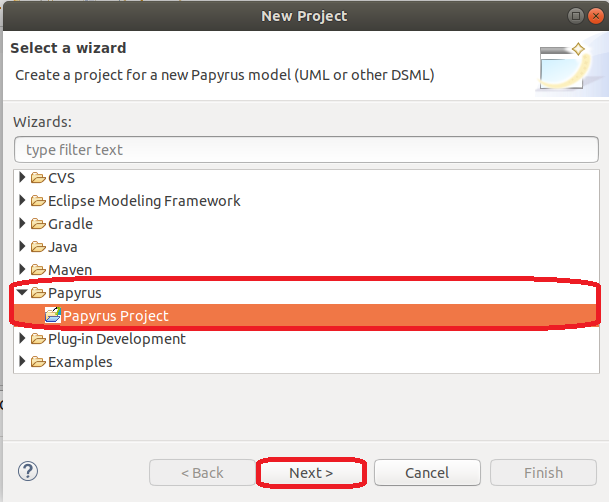
\includegraphics[scale=0.3]{./chapter4/javaCodesGeneration/Selection_001.png}}
\caption{Java Project Creation}
\label{fig:Java Project Creation}
\end{figure}

Once the Java project is created, its structure has to be modified in order to allow to be compatible with Maven. As the figure \ref{fig:Java Project Initial Structure} shows, firstly the Java project is composed of a JRE System Library and a src folder. This src folder has to be deleted, leaving the Java project only with the JRE System Library as it can be seen in the figure \ref{fig:Java Project Final Structure}.

\begin{figure}
\centering
{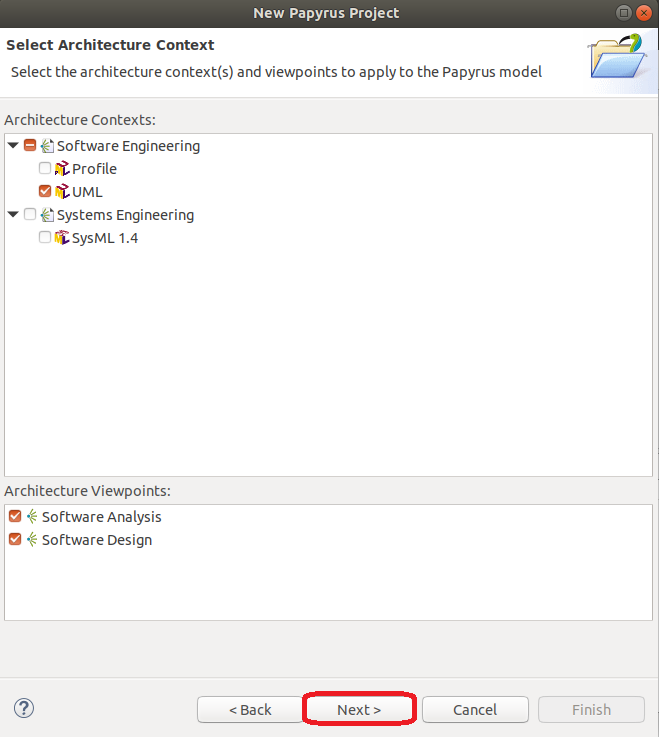
\includegraphics[scale=0.3]{./chapter4/javaCodesGeneration/Selection_002.png}}
\caption{Java Project Initial Structure}
\label{fig:Java Project Initial Structure}
\end{figure}

\begin{figure}
\centering
{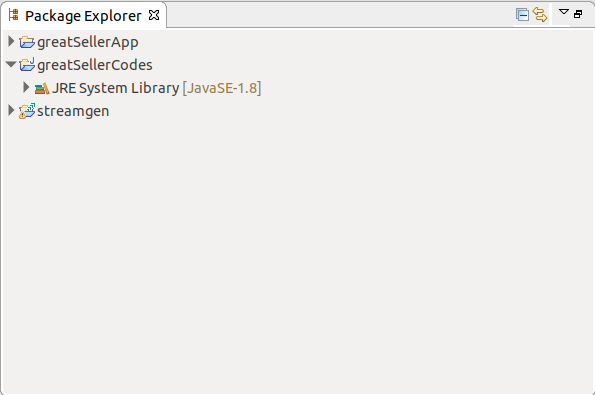
\includegraphics[scale=0.3]{./chapter4/javaCodesGeneration/Selection_003.png}}
\caption{Java Project Final Structure}
\label{fig:Java Project Final Structure}
\end{figure}

The next step is to create a source folder with a predefined structure as it is going to be specified now. Firstly, in the properties for the project, in the Java Build Path field, a folder has to added as the figure \ref{fig:Maven Project Structure Creation} specifies. In the default output folder a specific structure has to be written, greatSellerCodes/src/main/java. After this is written, the changes have to be applied and then click on 'Add Folder...'.

\begin{figure}
\centering
{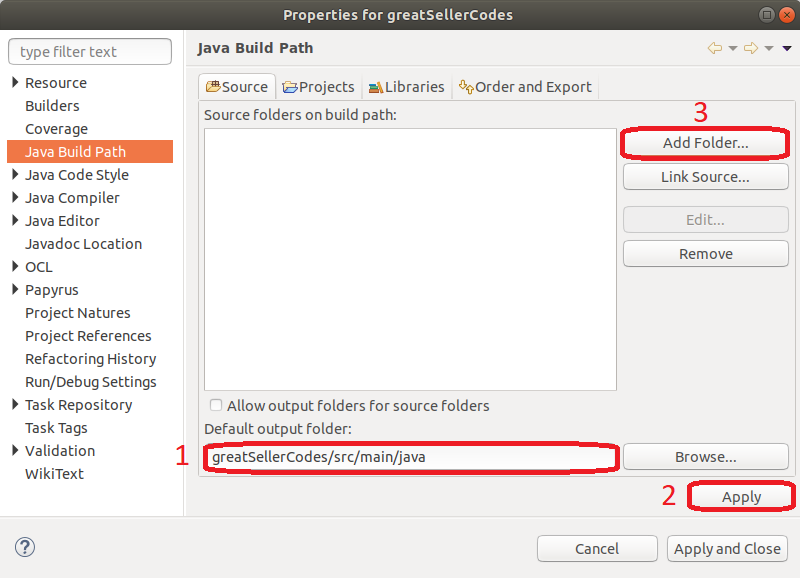
\includegraphics[scale=0.3]{./chapter4/javaCodesGeneration/Selection_004.png}}
\caption{Maven Project Structure Creation}
\label{fig:Maven Project Structure Creation}
\end{figure}

In order to create the source folder, the java folder has to be selected and then click on 'OK' as it is shown in figure \ref{fig:Maven Project Source Folder Creation}. Then the changes have to be applied and, then, the window Properties for greatSellerCodes has to be closed (figure \ref{fig:Maven Project Properties}).

\begin{figure}
\centering
{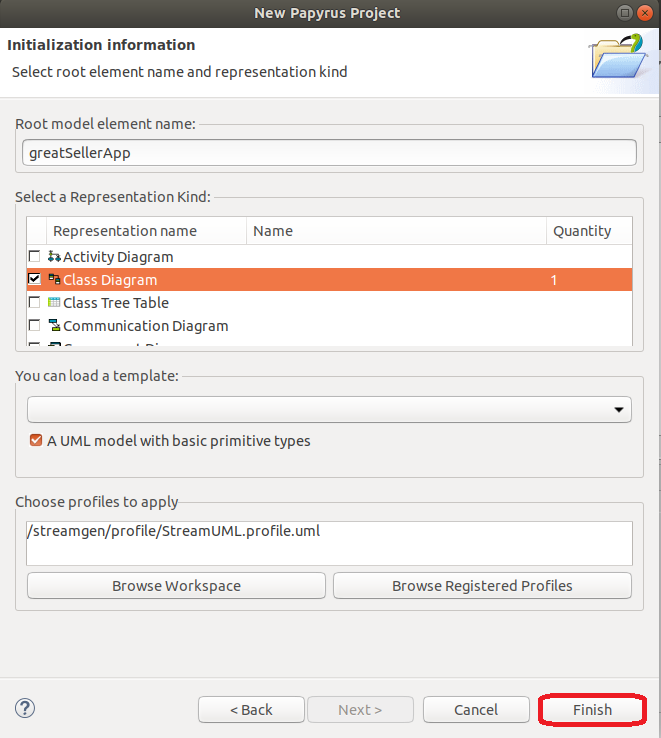
\includegraphics[scale=0.3]{./chapter4/javaCodesGeneration/Selection_005.png}}
\caption{Maven Project Source Folder Creation}
\label{fig:Maven Project Source Folder Creation}
\end{figure}

\begin{figure}
\centering
{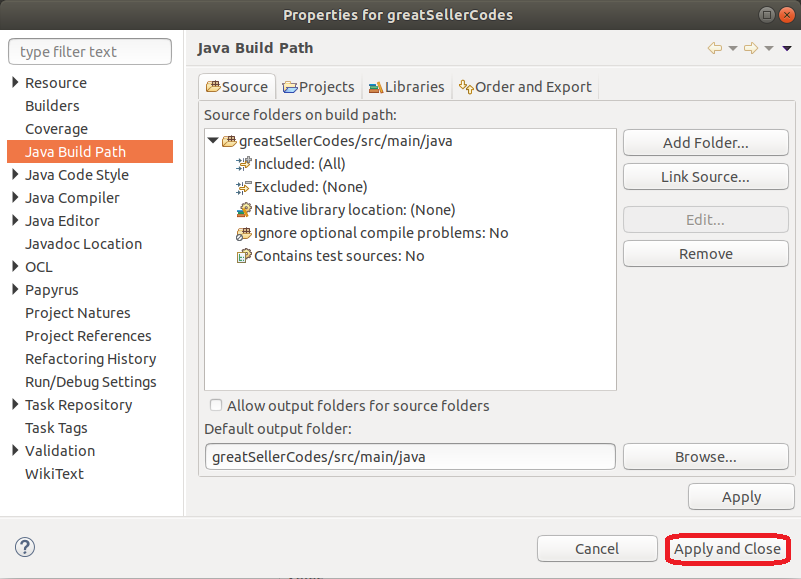
\includegraphics[scale=0.3]{./chapter4/javaCodesGeneration/Selection_006.png}}
\caption{Maven Project Properties}
\label{fig:Maven Project Properties}
\end{figure}

After these steps, the project folder should look like it is shown in the figure \ref{fig:Maven Project Structure} at the Package Explorer. And then, the project is ready to convert it into a Maven project. In order to do this, going to the 'Configure' option of the project and then clicking on 'Convert to Maven Project'. Then, a POM file has to be created and it is going to be created the default one as it can be seen in the figure \ref{fig:POM File Creation}. At this point, the structure of the project has to be the same that the one shown in the figure \ref{fig:Final Maven Project}.

\begin{figure}
\centering
{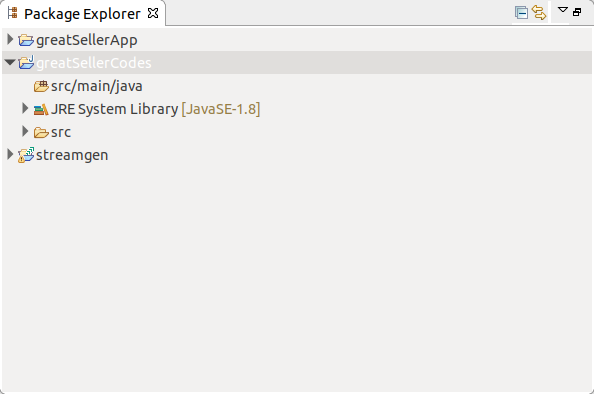
\includegraphics[scale=0.3]{./chapter4/javaCodesGeneration/Selection_007.png}}
\caption{Maven Project Structure}
\label{fig:Maven Project Structure}
\end{figure}

\begin{figure}
\centering
{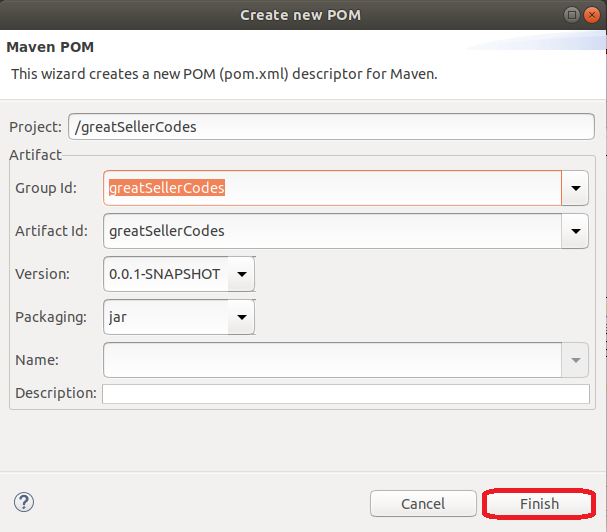
\includegraphics[scale=0.3]{./chapter4/javaCodesGeneration/Selection_008.png}}
\caption{POM File Creation}
\label{fig:POM File Creation}
\end{figure}

\begin{figure}
\centering
{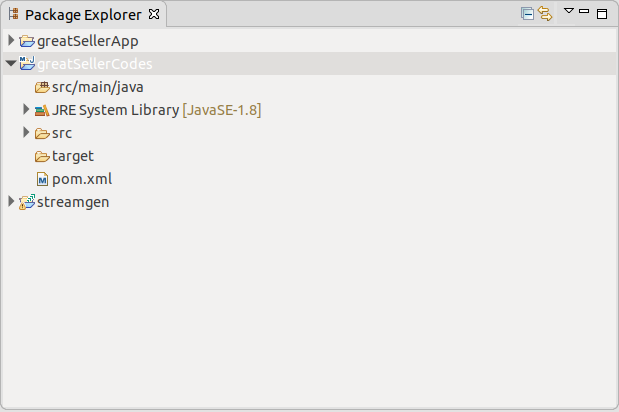
\includegraphics[scale=0.3]{./chapter4/javaCodesGeneration/Selection_009.png}}
\caption{Final Maven Project}
\label{fig:Final Maven Project}
\end{figure}

Now it is time to run the configuration (Run -$>$ Run Configurations...). In the figure \ref{fig:Run Configuration} is shown how this window has to be filled.

\begin{figure}
\centering
{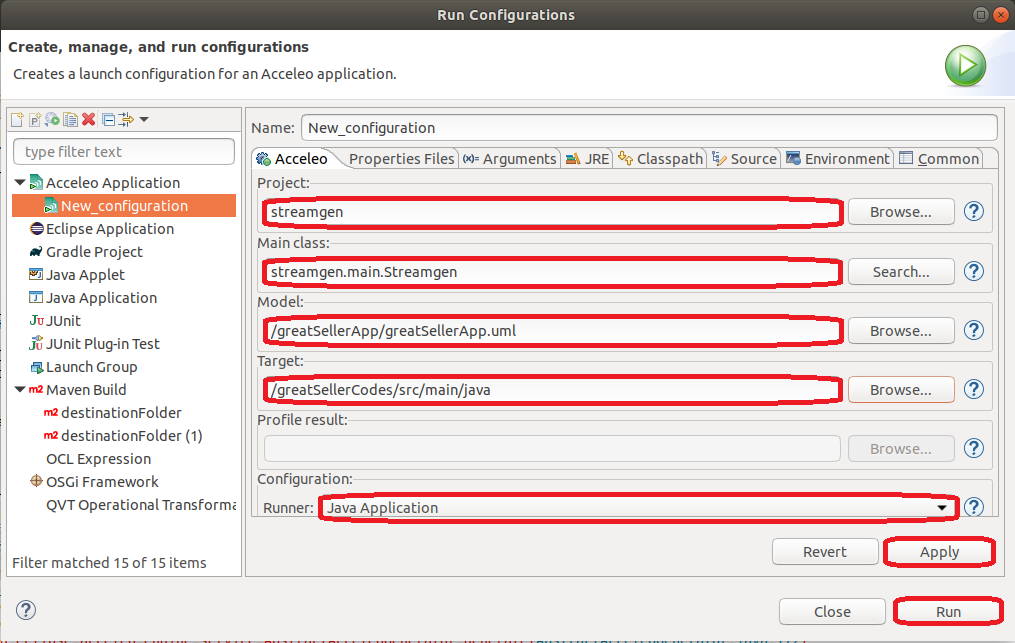
\includegraphics[scale=0.3]{./chapter4/javaCodesGeneration/Selection_010.png}}
\caption{Run Configuration}
\label{fig:Run Configuration}
\end{figure}
